\documentclass[style=upen, size=14pt]{powerdot}
\usepackage{natbib}
\usepackage{bibentry}
\usepackage{mathtools}
\definecolor{arany}{RGB}{255,242,0}
\hypersetup{backref=page}
\hypersetup{
    colorlinks=true,
    linkcolor=cyan,
    citecolor=cyan,
    filecolor=magenta,      
    urlcolor=cyan}
% \pdsetup{trans=Split}
\usepackage{graphicx}
\usepackage{amsmath}
\DeclareMathOperator*{\argmax}{argmax}
\DeclareMathOperator*{\argmin}{argmin}
\DeclareMathOperator*{\softmax}{softmax}
\DeclareMathOperator{\sign}{sign}
\usepackage{amssymb}
\usepackage{stmaryrd}
\usepackage[latin2]{inputenc}
%\usepackage[magyar]{babel}
%\usepackage{euler}
\usepackage{tikz}
\usetikzlibrary{matrix}
\usepackage{tikz-qtree}
\usepackage{tikz-dependency}
\usepackage{linguex}
\usepackage{amsthm}
\usepackage{amsmath}
%\tikzset{every tree node/.style={align=center,anchor=north}}
%\usepackage{tabularx}
%\usepackage{threeparttable}
%\usepackage{color}
%\selectlanguage{english}
%\frenchspacing
\usepackage{algpseudocode}
\usepackage{algorithm}
\newcommand\varlist{,\makebox[1em][c]{.\hfil.\hfil.},}
\newcommand{\nd}{\noindent}
\newcommand{\Val}{\mathop{\mathit{Val}}}
\newcommand{\gold}{\color{arany}}
%\usepackage{tikz}
%\usepackage{tikz-qtree}
%\newcommand{\qed}{\hfill\mbox{\raggedright \rule{.1in}{.1in}}}
\def\es{\mathbin\land}
\theoremstyle{definition}
\newtheorem*{definition}{Definition}
\newtheorem{axioma}{Axiom}
\newtheorem{tetel}{Theorem}
\newtheorem{prop}{Proposition}
\newtheorem{lemma}{Lemma}
\begin{document}

\title{Natural Language Processing\\~~\\Lecture 6\\Dependency parsing}
% \author{}

\date{2021}
\maketitle

\section{The dependency parsing task}

\begin{slide}[toc=Syntactic parsing]{Syntactic parsing (refresher)}
  Syntactic theories aim to characterize

  \begin{quote}
  ``the set of rules or principles that
  govern how words are put together to form phrases, well formed sequences of
  words.'' \citep[1]{koopman2013introduction}
\end{quote}

  The most important ``well formed sequences'' in this context are
  \emph{sentences}: the central goal of syntactic theories for a given language
  is to find structural rules or principles that characterize/delineate well
  formed sentences of the language in question.
\end{slide}

\begin{slide}[toc=]{Syntactic parsing cont.}
  A sentence is well formed if it has a \emph{structural description} or
  \emph{syntactic parse} which satisfies the syntactic constraints of the theory in
  question. Syntactic well formedness doesn't guarantee coherence or
  meaningfulness. To use Chomsky's famous example:
  
  \begin{quotation}
    \emph{Colorless green ideas sleep furiously.}
  \end{quotation}
  
  is syntactically well formed but nonsensical, while

  \begin{quotation}
    \emph{Furiously sleep ideas green colorless.}
  \end{quotation}

  is not even well formed.
\end{slide}

\begin{slide}[toc={Dep. grammars}]{Dependency grammars (refresher)}
  Dependency grammars treat the \emph{\gold dependency relation}
  between words as fundamental.

  The precise criteria vary from theory to theory,
  but typically a $d$ word depends on a $h$ word (equivalently, $h$ heads $d$)
  in a sentence if
  \begin{itemize}
  \item $d$ modifies the meaning of $h$, makes it more specific, e.g.
    \emph{eats} $\Rightarrow$ \emph{eats bread}, \emph{eats slowly} etc.
  \item and there is an asymmetric relationship of omissibility between them:
    $d$ can be omitted from the sentence keeping $h$ but not vice versa.
  \end{itemize}
\end{slide}

\begin{slide}[toc=]{Dependency grammars cont.}
  Dependency grammars impose important global constraints on the dependency
  relations within a well formed sentence:
  
  \begin{itemize}
  \item There is exactly one independent word (the root of the sentence).
  \item All other words depend directly on exactly one word.
  \end{itemize}
  As a consequence, the direct dependency graph of a sentence is a tree.

  Most dependency grammars work with \emph{typed direct dependencies}: there is
  finite list of direct dependency types with specific constraints on when they
  can hold.
\end{slide}


\begin{slide}[toc=]{Dependency grammars cont.}
  A dependency parse tree of the earlier example:
  \begin{center}
    \begin{dependency}[theme=simple, edge style={white}, label style={text=white}]
      \begin{deptext}[column sep=1em, nodes={text=white}]
        the \& students \& love \& their \& professors \\
      \end{deptext}
      \depedge{2}{1}{det}
      \depedge{3}{2}{nsubj}
      \depedge{3}{5}{dobj}
      \depedge{5}{4}{poss}
    \end{dependency}
  \end{center}
  Compared to the constituency tree, it contains fewer nodes (one per word), but
  the edges are labeled with the corresponding dependency types.
\end{slide}

\begin{slide}{Projectivity}
  An important (not always satisfied) requirement on dependency parse trees is 
  \emph{projectivity}:
  \begin{quote}
    If a $w$ word depends directly on $h$ and a $w'$ word lies between them in
    the sentence's word order, then the head of this $w'$ is either $w$ or $h$,
    or another word between them.
  \end{quote}
  Less formally, the projectivity condition states that dependencies are
  \emph{nested}, there cannot be \emph{crossing} dependencies between words.
\end{slide}

\begin{slide}[toc=]{Projectivity cont.}
    \begin{center}
      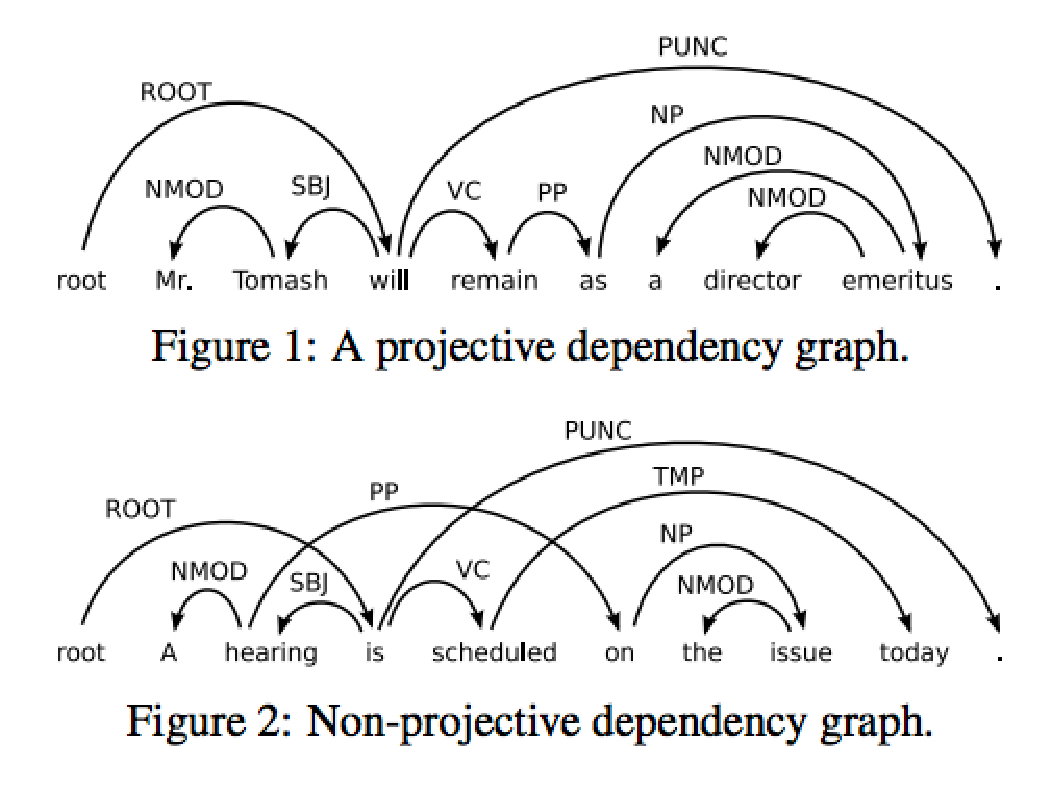
\includegraphics[width=0.85\textwidth]{figures/projectivity.eps}\\
      \footnotesize{(Figure from
        \href{https://languagelog.ldc.upenn.edu/nll/?p=7851}{Language Log:
          Non-projective flavor}.)}
  \end{center}
\end{slide}

\begin{slide}[toc=Dep. advantages]{The advantages of dependency grammars}
  Dependency grammars are becoming the dominant syntactic theory used in NLP,
  since
  \begin{itemize}
  \item dependency trees are in many respect simpler structures than phrase
    structure parse trees (e.g., have only one node per word);
  \item the predicate-argument analysis of sentences provided by dependency
    graphs is a very good starting point for event or frame-oriented semantic
    analysis.
  \end{itemize}
\end{slide}

\begin{slide}[toc=Semantic representation]{Usability for semantic
    representation}
  Compare, for event-semantic aspects
  \begin{small}
  \begin{center}
    \begin{dependency}[theme=simple, edge style={white}, label style={text=white}]
      \begin{deptext}[column sep=1em, nodes={text=white}]
        the \& students \& love \& their \& professors \\
      \end{deptext}
      \depedge{2}{1}{det}
      \depedge{3}{2}{nsubj}
      \depedge{3}{5}{dobj}
      \depedge{5}{4}{poss}
    \end{dependency}
    \Tree[.S [.NP [.Det \textit{the} ]
               [.Noun {\textit{students}} ]]
               [.VP [.Vt {\textit{love}} ]
               [.NP [.Det \textit{their} ]
               [.Noun {\textit{professors}} ]
             ]]]
           \end{center}
         \end{small}
\end{slide}

\begin{slide}[toc=The parsing task]{The dependency parsing task}
  Given a syntactic theory, the parsing task is to assign syntactic structure to
  input sentences which satisfy the constraints/conditions of the theory. For
  dependency grammars, this means assigning a \emph{dependency structure}:
  \begin{itemize}
  \item identifying direct dependencies between words of the sentence,
  \item in such a way that together they constitute a \emph{dependecy tree}
    which satisfies all of the the theory's constraints.
  \end{itemize}
\end{slide}

\begin{slide}[toc=]{The dependency parsing task cont.}
  In modern NLP practice, the dependency grammar underlying a parsing task is
  typically specified implicitly, using a so called \emph{\gold treebank}, that
  is, a dataset consisting of sentences annotated with their parse
  trees.\bigskip

  This makes parsing a \emph{\gold structured supervised learning task}: given a
  training set consisting of a large number of
  $\langle \mathrm{sentence}, \mathrm{parse}~\mathrm{tree} \rangle$ pairs, learn
  to predict the parse tree of unseen sentences.
\end{slide}

\begin{slide}{Performance metrics}
  For dependency grammar parsers, the most commonly used evaluation metrics are
  \begin{itemize}
  \item \emph{\gold UAS (Unlabeled Attachment Score):} The percentage of words that are
    attached to the correct head.
  \item \emph{\gold LAS (Labeled Attachment Score):} The percentage of words that are
    attached to the correct head with the correct dependency label.
  \end{itemize}
\end{slide}

\section{References}

\begin{slide}{References}
  \bibliographystyle{plainnat}
  \nobibliography{nlp_course.bib}
  \begin{footnotesize}

    \bibentry{koopman2013introduction}.\medskip


  \end{footnotesize}
\end{slide}

% \begin{slide}[toc=]{References cont.}
%   \begin{footnotesize}
    
%     \bibentry{murphy2021pml}\medskip
    
%   \end{footnotesize}
% \end{slide}

\end{document}

%%% Local Variables:
%%% mode: latex 
%%% TeX-master: t
%%% End:

% LocalWords:  Tokenization Discriminative discriminative
